% =============================================================================
%  Smile Labs - Data Storm v7.0 Final Round
%  Comprehensive Methodology & Technical Paper (max 10 pages)
%  Compile: pdflatex final_round_report.tex  (run twice for refs)
% =============================================================================
\documentclass[10pt,a4paper]{article}

\usepackage[utf8]{inputenc}
\usepackage[T1]{fontenc}
\usepackage{lmodern}
\usepackage[a4paper,margin=0.85in]{geometry}
\usepackage{graphicx}
\usepackage{amsmath,amssymb}
\usepackage{xcolor}
\usepackage{titlesec}
\usepackage{fancyhdr}
\usepackage{booktabs}
\usepackage{tabularx}
\usepackage{array}
\usepackage{enumitem}
\usepackage{float}
\usepackage{caption}
\usepackage{subcaption}
\usepackage[colorlinks=true,linkcolor=primary,urlcolor=primary,citecolor=primary]{hyperref}

\graphicspath{{figures/}}

% --- palette ------------------------------------------------------------------
\definecolor{primary}{RGB}{0,90,170}
\definecolor{accent}{RGB}{200,70,25}
\definecolor{green}{RGB}{31,140,75}
\definecolor{panelbg}{RGB}{238,244,250}
\definecolor{rulec}{RGB}{180,200,220}

% --- headers ------------------------------------------------------------------
\pagestyle{fancy}
\fancyhf{}
\fancyhead[L]{\small\textcolor{gray}{Smile Labs \,|\, Data Storm 7.0 -- Final Round}}
\fancyhead[R]{\small\textcolor{gray}{Latent Potential \& Spend Allocation}}
\fancyfoot[C]{\small\thepage}
\renewcommand{\headrulewidth}{0.4pt}
\renewcommand{\footrulewidth}{0pt}

% --- section styling ----------------------------------------------------------
\titleformat{\section}{\large\bfseries\color{primary}}{\thesection}{0.6em}{}
\titleformat{\subsection}{\normalsize\bfseries\color{primary!85!black}}{\thesubsection}{0.5em}{}
\titlespacing*{\section}{0pt}{1.0em}{0.4em}
\titlespacing*{\subsection}{0pt}{0.7em}{0.25em}

\captionsetup{font=small,labelfont={bf,color=primary},skip=3pt}
\setlength{\parindent}{0pt}
\setlength{\parskip}{0.45em}
\renewcommand{\arraystretch}{1.15}

% --- callout panel ------------------------------------------------------------
\newcommand{\panel}[2]{%
  \begin{center}\colorbox{panelbg}{%
  \begin{minipage}{0.96\linewidth}\vspace{2pt}
  {\bfseries\color{primary}#1}\\[1pt]\small #2
  \vspace{3pt}\end{minipage}}\end{center}}

\newcolumntype{Y}{>{\raggedright\arraybackslash}X}

\begin{document}

% =============================================================================
%  TITLE
% =============================================================================
\begin{center}
{\LARGE\bfseries\color{primary} Latent Outlet Potential \&\\[2pt]
Potential-Based Trade Spend Allocation}\\[6pt]
{\large Data Storm v7.0 -- Final Round}\\[2pt]
{\normalsize Sri Lanka \,$\cdot$\, January 2026 horizon}\\[6pt]
\rule{0.55\textwidth}{0.4pt}\\[5pt]
{\large\bfseries Submitted by Smile Labs}\\[2pt]
{\small Powered by OCTAVE -- John Keells Group \,|\, Rotaract Club of University of Moratuwa}
\end{center}
\vspace{2pt}

\panel{One-line method}{%
We estimate $\mathbb{E}[\text{true\_demand}_i \mid X_i]$ where observed sales
$y_i=\min(\text{true\_demand}_i,\text{constraint}_i)$ are \emph{right-censored}.
The estimand is \emph{not point-identified} from observational data alone, so we
report a $[\text{lower},\text{point},\text{upper}]$ band per outlet -- the point
combining Stochastic Frontier Analysis, multi-quantile gradient-boosted
regression, Chernozhukov--Hong censoring correction, Conformalised QR, and
bootstrap peer-bucket caps. On top of these predictions we add a \textbf{decision
layer}: a Lagrangian water-filling optimizer for the LKR\,5M Western budget, a
functional LLM-based Explainable-AI module, and an interactive Outlet
Intelligence web app.}

\begin{table}[H]
\centering\small
\begin{tabularx}{\textwidth}{Yr}
\toprule
\textbf{Headline} & \textbf{Value}\\
\midrule
Outlets predicted (full population in scope) & \textbf{20,000}\\
External POIs scraped (Geofabrik PBF, 9 categories) & \textbf{42,386}\\
Outlets with $\ge 1$ POI within 2\,km & 80.9\,\%\\
Rejected check records (coords + txn + holidays) & 10,179 / 3 datasets\\
Median uplift vs. historical max & \textbf{1.250$\times$}\\
Submission preflight (6 automated checks) & \textbf{6 / 6 PASS}\\
LKR\,5M Western budget -- outlets funded & 3,729 / 9,000\\
Expected incremental volume (Western) & \textbf{+109,021\,L}\\
Revenue-to-spend ROI & \textbf{5.53$\times$}\\
\bottomrule
\end{tabularx}
\caption{Headline value across prediction and decision layers.}
\end{table}

\panel{Build trail}{The modeling stack was built and audited across
\textbf{seven rounds of AI council reviews} (four parallel premium-model critics
per round). Every fix in \texttt{src/} cites the council finding it addresses
(\texttt{FIX R7}, \texttt{FIX R4}, \texttt{FIX M1}, \dots). Provenance:
\texttt{Reviews/} and \texttt{Docs/ai\_transparency\_log.md}.}

% =============================================================================
\section{Data Engineering and Scraping Pipeline}

\subsection{Bronze $\rightarrow$ Silver $\rightarrow$ Gold lakehouse}
Raw CSVs ingest \emph{as-is} into \texttt{data/bronze/} with a SHA-256 audit log
(idempotent: re-runs overwrite deterministically and re-hash). The \textbf{Silver}
layer applies six reusable, parameterizable data-quality functions
(\texttt{src/quality/checks.py}) consistently across all five raw datasets; failed
rows are quarantined to \texttt{data/silver\_rejected/} carrying
\texttt{dataset\_name}, \texttt{failed\_check}, and \texttt{failure\_reason}.
\textbf{Gold} is the model-ready outlet\,$\times$\,feature parquet.

\begin{figure}[H]
\centering
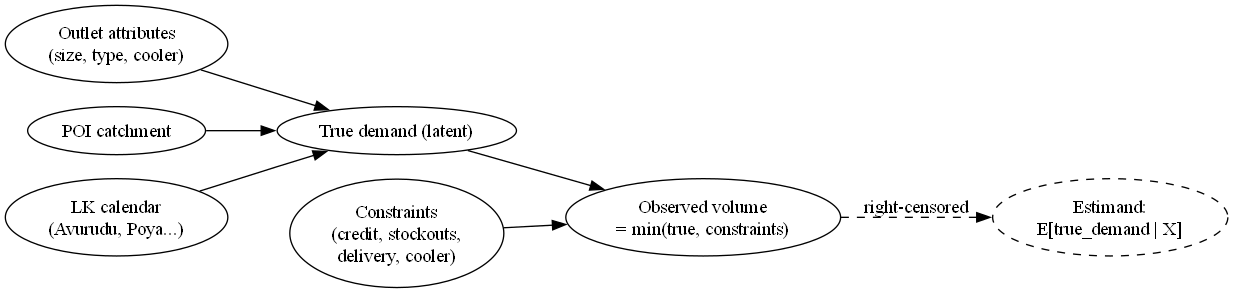
\includegraphics[width=0.78\textwidth]{dag.png}
\caption{Bronze $\rightarrow$ Silver $\rightarrow$ Gold pipeline and the
right-censoring DAG: observed sales are the $\min$ of latent demand and
constraint, so the estimand is only partially identified.}
\end{figure}

\subsection{POI acquisition: Geofabrik PBF $\gg$ na\"ive Overpass}
Na\"ively querying Overpass for $20{,}000\times 9\text{ cats}\times 4\text{ radii}
=720{,}000$ requests is infeasible (timeouts + ToS). We instead download the
\textbf{Geofabrik Sri Lanka extract} (\texttt{sri-lanka-latest.osm.pbf},
$\sim$136\,MB) once, parse locally with \texttt{pyrosm}, and run nearest-neighbour
search via \texttt{BallTree(metric="haversine")}. End-to-end 25--45\,min, offline
after one fetch. Lives in \texttt{poi\_pipeline/} as an idempotent sub-project.

\begin{table}[H]
\centering\footnotesize
\begin{tabularx}{\textwidth}{lrY}
\toprule
\textbf{Category} & \textbf{POIs} & \textbf{OSM tags}\\
\midrule
Schools / universities & 5,694 & \texttt{amenity} $\in$ \{school, university, college\}\\
Transport hubs & 5,799 & \texttt{highway=bus\_stop}, \texttt{railway=station}\\
Hospitals + healthcare & 2,007 & \texttt{amenity} $\in$ \{hospital, clinic, pharmacy\}\\
Restaurants / cafes & 4,667 & \texttt{amenity} $\in$ \{restaurant, cafe, fast\_food\}\\
Supermarkets / groceries & 2,543 & \texttt{shop} $\in$ \{supermarket, convenience\}\\
Religious places & 9,255 & \texttt{amenity=place\_of\_worship}\\
Hotels / attractions & 5,513 & \texttt{tourism} $\in$ \{hotel, guest\_house\}\\
Offices & 4,169 & \texttt{office=*}, \texttt{amenity=townhall}\\
Banks / ATMs & 2,739 & \texttt{amenity} $\in$ \{bank, atm\}\\
\midrule
\textbf{Total} & \textbf{42,386} & 80.9\,\% outlets with $\ge1$ POI within 2\,km\\
\bottomrule
\end{tabularx}
\caption{POI extraction summary (\texttt{poi\_pipeline/data/pois/}).}
\end{table}

\subsection{Features for footfall and market potential}
\textbf{Spatial distance-decay (\S2.1).} Each category contributes a
Gaussian-decay catchment score so a bus stop 20\,m away dominates one 400\,m away:
\[
\text{score}_{i,c}=\sum_{p\in c}\exp\!\Big(-\tfrac{d(i,p)^2}{2\sigma_c^2}\Big),
\]
with $d$ the haversine distance and $\sigma_c$ a category bandwidth; the nine
scores are z-averaged into \texttt{poi\_catchment\_score}.

\textbf{Competitive catchment density (\S2.2).} We count outlets within 500\,m
(\texttt{competitor\_count\_500m}) and 1/2/5\,km, plus
\texttt{same\_distributor\_outlet\_count\_5km},
\texttt{nearest\_outlet\_distance\_km}, and \texttt{cannibalisation\_count\_200m},
normalised into \texttt{competitive\_intensity}$\in[0,1]$ separating a crowded
cluster from an untapped market.

\textbf{Honest disclosure.} Per-outlet POI counts correlate only weakly with
volume ($|r|\le0.026$ across \texttt{Outlet\_Type} groups), so POI enters
\emph{only} via the composite score at $\sim$20\,\% weight in the constraint score
-- never as a standalone predictor. We flag the OSM-LK mapping bias: small kades
and roadside stalls (our targets) are under-mapped.

\begin{figure}[H]
\centering
\begin{subfigure}{0.49\textwidth}\centering
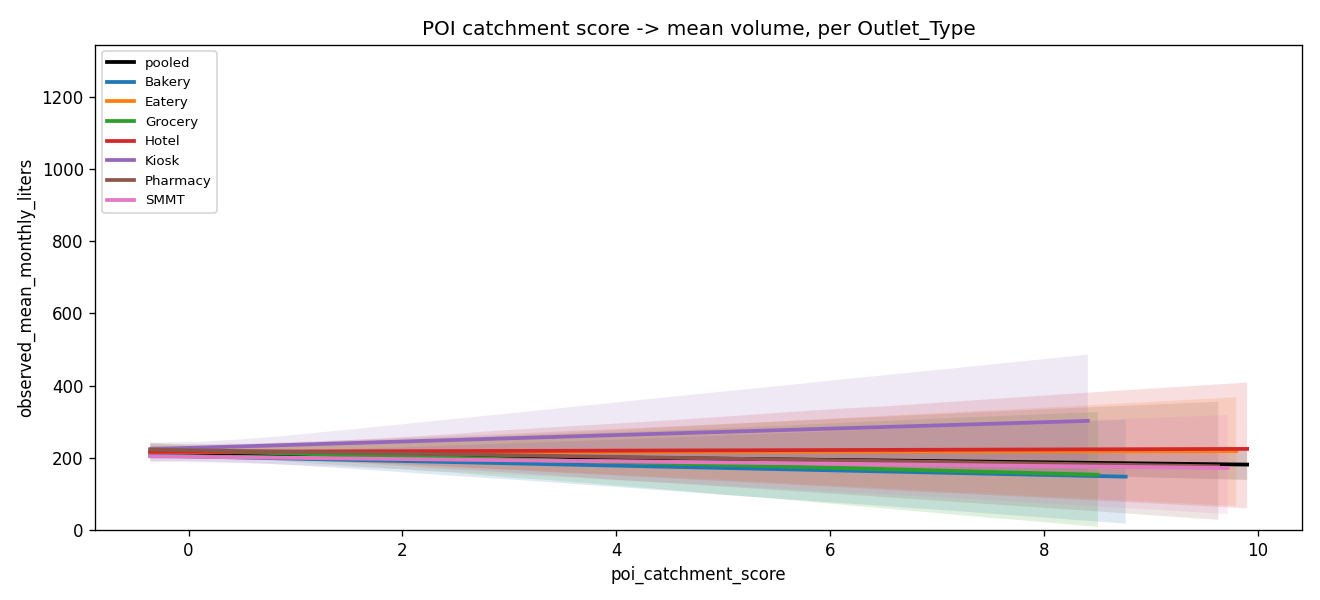
\includegraphics[width=\textwidth]{eda_poi_outlet_type.png}
\caption{POI catchment is a \emph{location} signal, not a direct predictor.}
\end{subfigure}\hfill
\begin{subfigure}{0.49\textwidth}\centering
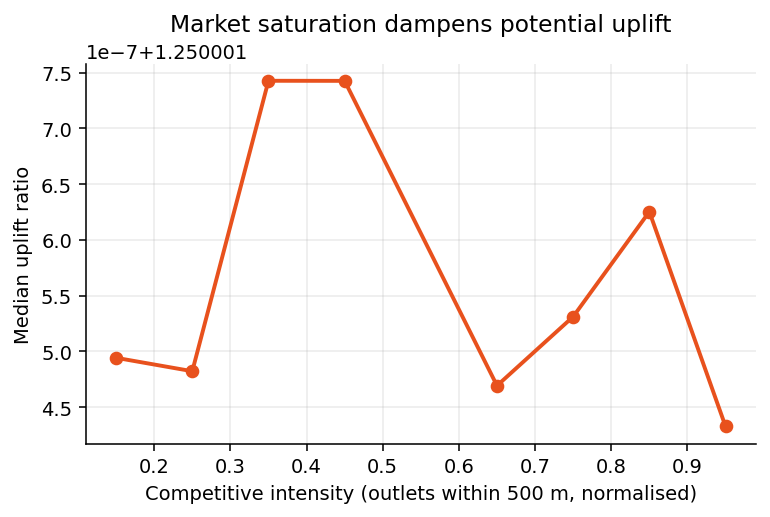
\includegraphics[width=\textwidth]{fr_competition_effect.png}
\caption{Denser competition $\Rightarrow$ lower median uplift (saturation).}
\end{subfigure}
\caption{External-data signals: POI catchment (left) and competitive saturation (right).}
\end{figure}

% =============================================================================
\section{Data Cleaning}

\subsection{Initial quality assessment -- six reusable checks}
\begin{table}[H]
\centering\small
\begin{tabularx}{\textwidth}{lY}
\toprule
\textbf{Function (\texttt{checks.py})} & \textbf{What it catches}\\
\midrule
\texttt{duplicate\_check(df, key\_columns)} & duplicate composite keys\\
\texttt{null\_check(df, columns)} & NaN / empty mandatory fields\\
\texttt{range\_check(df, col, min, max)} & numeric out-of-range\\
\texttt{domain\_check(df, col, allowed)} & misspellings, unexpected enums\\
\texttt{referential\_integrity\_check(\dots)} & foreign keys not in master\\
\texttt{geospatial\_bounds\_check(\dots)} & coordinates outside Sri Lanka\\
\bottomrule
\end{tabularx}
\caption{All six DQ functions are parameterised and reused across datasets.}
\end{table}

\subsection{Programmatic cleaning \& artifact neutralisation}
\begin{table}[H]
\centering\footnotesize
\begin{tabularx}{\textwidth}{Yrl}
\toprule
\textbf{Artifact} & \textbf{Records} & \textbf{Action}\\
\midrule
\texttt{Outlet\_Type} typos + \texttt{Outlet\_Size} case/missing & 1,581 & normalised / \texttt{Unknown}\\
Coordinates outside Sri Lanka (5.5--10$^\circ$N) & 240 & quarantined\\
Non-positive \texttt{Volume\_Liters} / \texttt{Bill\_Value} & 9,606 & quarantined\\
Holiday duplicates (date+name+type) & 93 & deduped to rejected\\
\bottomrule
\end{tabularx}
\caption{Every quarantined row carries a documented \texttt{failure\_reason}
(\texttt{src/cleaning/silver.py}).}
\end{table}

\subsection{Capacity from a measured saturation knee}
Volume \emph{stops growing} after 3 coolers (notebook 23): median monthly volume
at 3, 4 and 5+ coolers is statistically indistinguishable. We use
\texttt{Cooler\_Count} as the deterministic sign anchor for the PCA capacity
component -- a physical representation of the cooler-replenishment ceiling.

\begin{figure}[H]
\centering
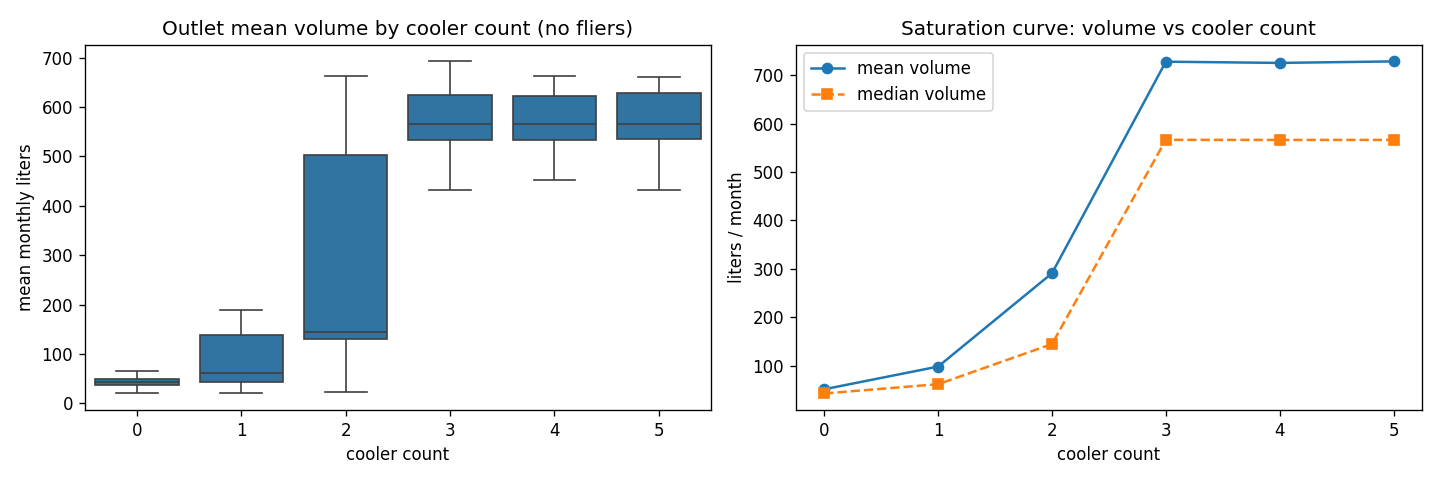
\includegraphics[width=0.62\textwidth]{eda_cooler_saturation.png}
\caption{Saturation knee at 3 coolers anchors the capacity feature.}
\end{figure}

% =============================================================================
\section{The Mathematical Framework}

\subsection{Identification: right-censored, not point-identified}
The estimand $\mathbb{E}[\text{true\_demand}_i\mid X_i]$ is \textbf{not
point-identified} from observational data (no exogenous variation in
constraints). $y_i=\min(\text{true\_demand}_i,\text{constraint}_i)$ is
right-censored -- for any constrained outlet we see only a lower bound. We report
a \emph{band} alongside the point. For 15.62\,\% of outlets the q90 frontier lies
\emph{below} observed historical max; without a $\max(\cdot,\text{obs\_max})$
floor, validation V3b fails for those rows.

\begin{figure}[H]
\centering
\begin{subfigure}{0.49\textwidth}\centering
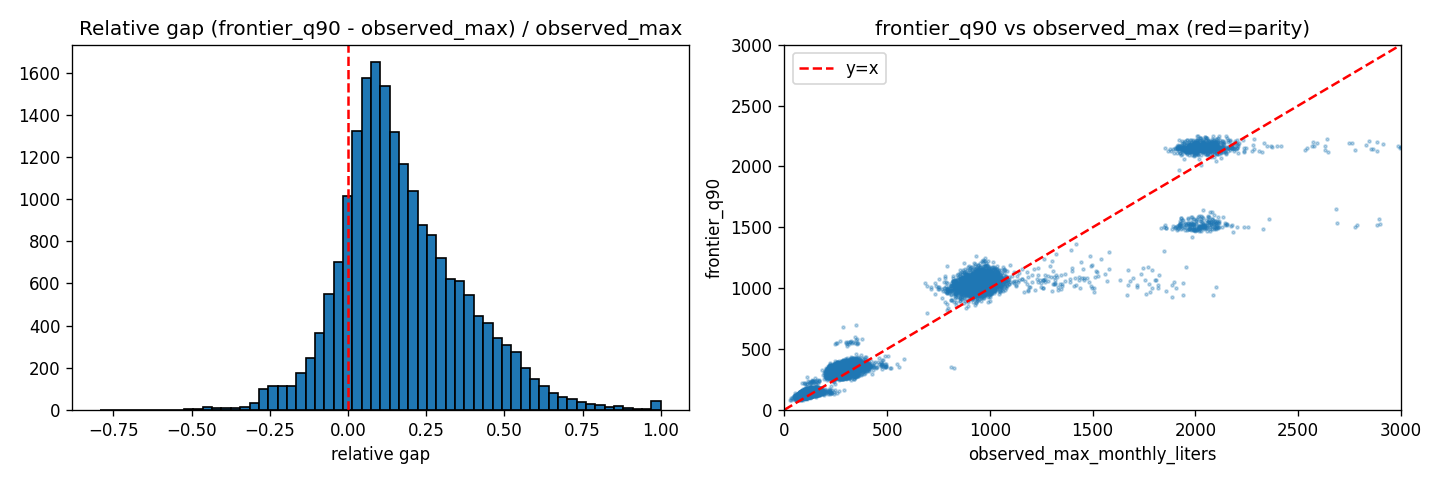
\includegraphics[width=\textwidth]{eda_frontier_gap.png}
\caption{Negative frontier gap motivates the \texttt{obs\_max} floor.}
\end{subfigure}\hfill
\begin{subfigure}{0.49\textwidth}\centering
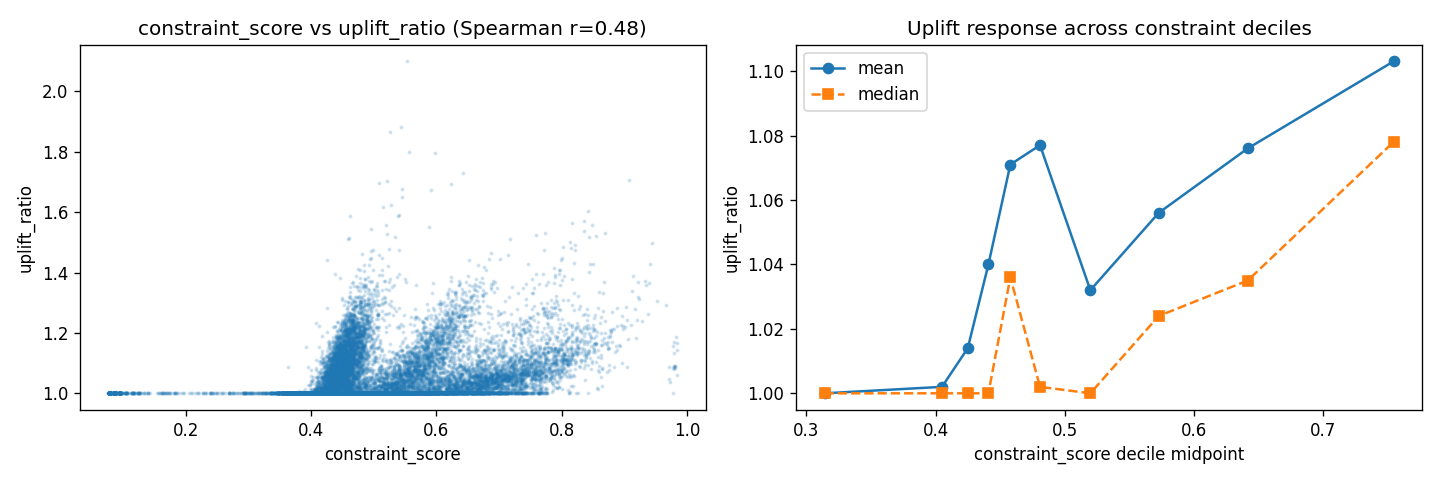
\includegraphics[width=\textwidth]{eda_constraint_uplift.png}
\caption{Constraint score drives per-outlet uplift, capped by evidence.}
\end{subfigure}
\caption{Censoring evidence (left) and the constraint-to-uplift mechanism (right).}
\end{figure}

\subsection{Method stack}
\textbf{Robust lower bound + frontier ensemble.}
$\text{lower}_i=\max(\text{3rd-highest month}_i,\ \text{median}_i)$. The frontier
$F_i$ is a 60/40 blend of (a) \textbf{XGBoost 2.0} with \texttt{reg:quantileerror},
\texttt{quantile\_alpha=[0.5,0.75,0.9,0.95]}, monotone constraints + isotonic
post-sort, and (b) \textbf{SFA}: $y=X\beta+v-u$ with truncated-normal $u$, direct
MLE; per-outlet $\text{TE}=\exp(-\mathbb{E}[u\mid\varepsilon])$ ($\sigma_v\approx
0.41$, $\sigma_u\approx0.78$, $\lambda\approx1.92$; median TE $\approx0.84$).
Leaky \texttt{observed\_*} aggregates are dropped from the SFA design matrix.

\textbf{Censoring correction + constraint score.} Chernozhukov--Hong (2002) 3-step:
a propensity $P(\text{censored}\mid X)$ on plateau proxies, then q90 refit on
$P<0.10$ (only 1.16\,\% of outlets show a true plateau -- a small-population
correction). The constraint score $s_i\in[0,1]$ blends three \emph{orthogonal}
signals: peer-q90 frontier residual z-score, plateau gate, PCA-decorrelated
capacity.

\textbf{Final formula + calibrated interval.}
\[
\text{potential}_i=\max\!\Big(\text{obs\_max}_i,\ \text{lower}_i+s_i(F_i-\text{lower}_i),\
\mathbf{1}_{[s_i\ge0.4]}\cdot1.25\cdot\text{obs\_max}_i\Big)
\ \text{capped at}\ B_i\cdot\text{obs\_max}_i,
\]
where $B_i$ is the empirical 95th-pct uplift inside outlet $i$'s
(\texttt{Outlet\_Type}$\times$\texttt{Outlet\_Size}) bucket. We additionally report
a calibrated $[q_{05},q_{95}]$ via \textbf{Conformalised QR} on a 20\,\%
outlet-level holdout, plus \textbf{Manski} worst-case bounds.

\begin{figure}[H]
\centering
\begin{subfigure}{0.49\textwidth}\centering
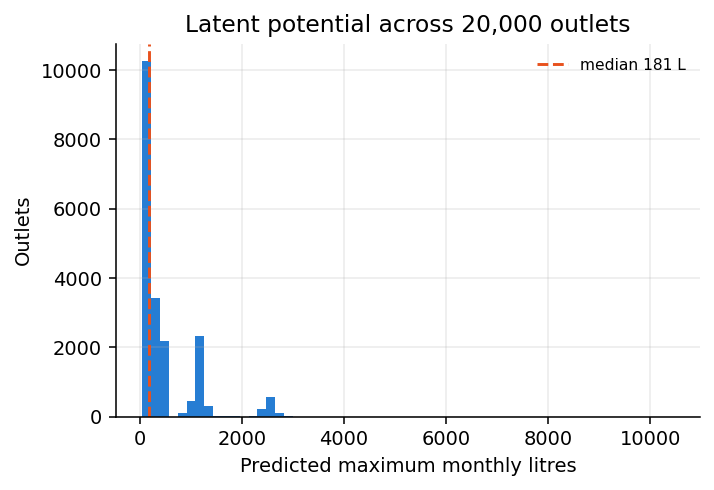
\includegraphics[width=\textwidth]{fr_potential_dist.png}
\caption{Latent potential across 20,000 outlets.}
\end{subfigure}\hfill
\begin{subfigure}{0.49\textwidth}\centering
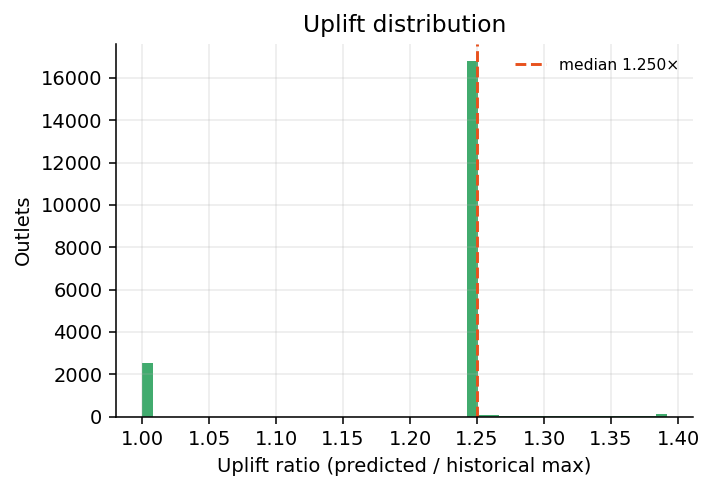
\includegraphics[width=\textwidth]{fr_uplift_dist.png}
\caption{Uplift ratio; median 1.250$\times$, no implausible tail.}
\end{subfigure}
\caption{Prediction outputs: potential (left) and uplift distribution (right).}
\end{figure}

% =============================================================================
\section{Spend Optimization Logic}

\textbf{Problem.} Distribute a fixed \textbf{LKR\,5,000,000} Western budget across
the 9,000 Western outlets (\texttt{DIST\_W\_01/02/03}) to \emph{maximise additional
sales volume} over the normal baseline, with total spend $\le$ budget. Western
holds the largest untapped headroom of the four provinces.

\textbf{Response model (concave, saturating).} Incremental litres from spend $s$:
$g_i(s)=H_i(1-e^{-s/k_i})$, where $H_i$ is latent headroom and the responsiveness
scale grows with revenue value and competition:
$k_i=\alpha(H_i\cdot\text{bill\_per\_litre}_i)(1+\beta\,\text{comp\_intensity}_i)$.
A revenue-anchored cap $\text{cap\_frac}\cdot H_i\cdot\text{bill}_i$ prevents a few
large outlets from absorbing the budget ($\alpha{=}0.15,\beta{=}0.50,
\text{cap\_frac}{=}0.35$).

\textbf{Exact solution -- Lagrangian water-filling (KKT).} Since
$\sum_i g_i(s_i)$ is separable-concave, the optimum is exact. Stationarity gives
$g_i'(s_i^\star)=\lambda$, and with $g_i'(s)=\tfrac{H_i}{k_i}e^{-s/k_i}$ each spend
is closed-form in the shadow price:
$s_i^\star(\lambda)=\big[k_i\ln(\tfrac{H_i}{k_i\lambda})\big]_0^{\text{cap}_i}$.
We \textbf{bisect on $\lambda$} until $\sum_i s_i^\star=B$ (budget-feasible,
optimal) -- not a heuristic ranking.

\begin{table}[H]
\centering\small
\begin{tabularx}{0.92\textwidth}{Yr}
\toprule
\textbf{Metric (Western, LKR 5M, Jan 2026)} & \textbf{Value}\\
\midrule
Budget utilisation & 98.0\,\% (LKR 4,901,675)\\
Outlets funded & 3,729 / 9,000\\
Expected incremental volume & \textbf{+109,021\,L}\\
Expected incremental revenue & LKR 27.08\,M\\
Litres per LKR 1,000 (blended) & 21.8\,L\\
Revenue-to-spend ROI & \textbf{5.53$\times$}\\
\bottomrule
\end{tabularx}
\caption{\texttt{Results/budget\_allocation\_summary.json}. Submission:
\texttt{smile\_labs\_budget\_allocations.csv}.}
\end{table}

The allocation concentrates spend on \textbf{high-headroom, high-margin,
moderately-competitive} outlets -- most untapped potential per rupee -- rather
than rewarding saturated top sellers or starving isolated shops.

\begin{figure}[H]
\centering
\begin{subfigure}{0.49\textwidth}\centering
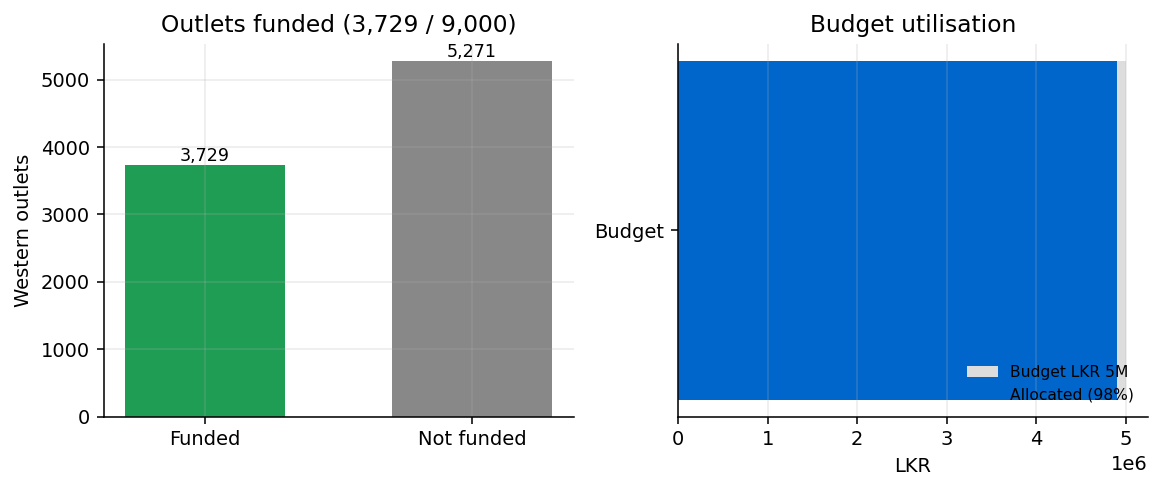
\includegraphics[width=\textwidth]{fr_allocation_summary.png}
\caption{3,729 of 9,000 funded; 98\,\% of budget used.}
\end{subfigure}\hfill
\begin{subfigure}{0.49\textwidth}\centering
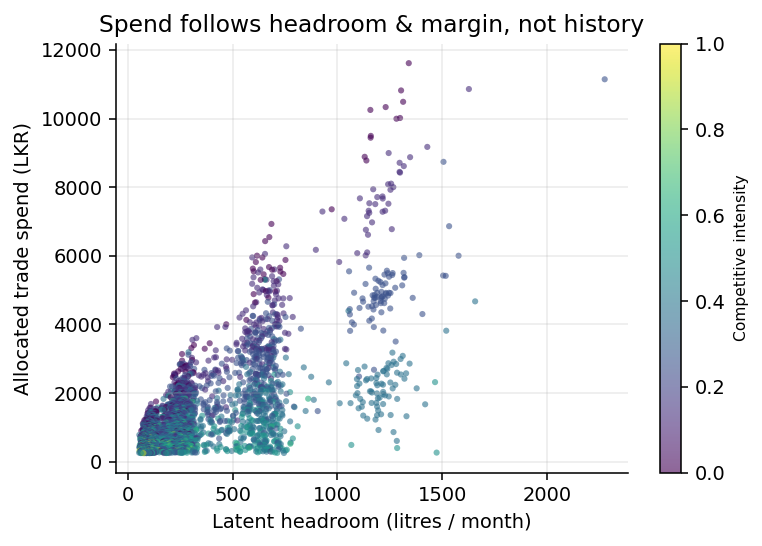
\includegraphics[width=\textwidth]{fr_spend_vs_headroom.png}
\caption{Spend tracks headroom \& margin, modulated by competition.}
\end{subfigure}

\vspace{4pt}
\begin{subfigure}{0.49\textwidth}\centering
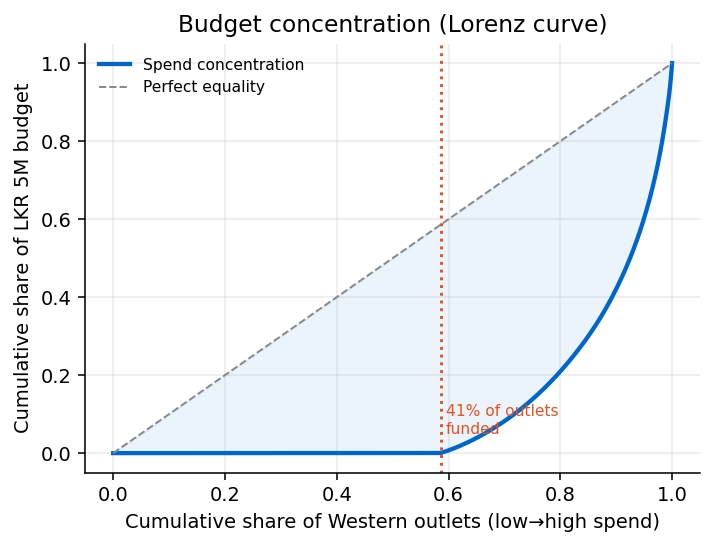
\includegraphics[width=\textwidth]{fr_spend_lorenz.png}
\caption{Lorenz curve: budget concentrated on highest-return outlets.}
\end{subfigure}\hfill
\begin{subfigure}{0.49\textwidth}\centering
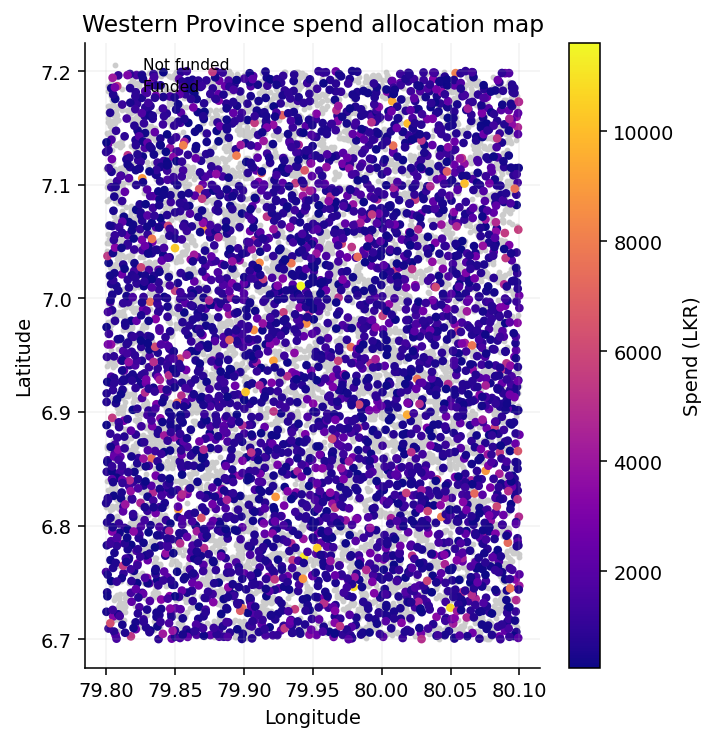
\includegraphics[width=\textwidth]{fr_western_spend_map.png}
\caption{Geographic Western allocation (funded coloured by spend).}
\end{subfigure}
\caption{Spend optimization outputs: utilisation, mechanism, concentration, and geography.}
\end{figure}

% =============================================================================
\section{Functional Explainable AI (XAI)}
The XAI module (\texttt{src/xai/}) is a \textbf{user-facing layer} embedded in the
web app, in two stages mapped to the four signal groups the brief requires.

\begin{enumerate}[leftmargin=1.3em,itemsep=1pt]
\item \textbf{\texttt{drivers.py} -- signed driver payload.} Converts a prediction
into a ranked, signed set of drivers: \emph{model drivers} (latent headroom,
best-month anchor, history depth), \emph{local signals} (competitive density, POI
intensity), and \emph{operational constraints} (cooler capacity vs the size norm).
Each carries a direction, a relative weight, and a one-line technical detail.
\item \textbf{\texttt{narrative.py} -- LLM narrative.} An LLM translates the
payload into plain business language (why this score, which factors moved it, how
local conditions shaped it). Uses the \textbf{Anthropic API}
(\texttt{claude-opus-4-8}) when \texttt{ANTHROPIC\_API\_KEY} is set, with a
deterministic \textbf{offline fallback}. Both paths consume the same structured
payload, so narratives are validated against the drivers, never free-floating
(samples in \texttt{Results/xai\_samples.json}).
\end{enumerate}

% =============================================================================
\section{Validation, Outputs \& Web App}

\subsection{Validation without ground truth (6-item checklist)}
\begin{table}[H]
\centering\small
\begin{tabularx}{\textwidth}{clYc}
\toprule
\textbf{\#} & \textbf{Check} & \textbf{Detail (final run)} & \textbf{Status}\\
\midrule
V1 & schema + row count & \texttt{[Outlet\_ID, Max\_Monthly\_Liters]}, 20,000 & \textcolor{green}{\textbf{OK}}\\
V2 & no NaN/neg, unique IDs & NaN=0, neg=0, unique=True & \textcolor{green}{\textbf{OK}}\\
V3a & every ID in outlet\_master & missing = 0 & \textcolor{green}{\textbf{OK}}\\
V3b & pred $\ge$ hist.\ max ($\ge99\%$) & 0.00\,\% below & \textcolor{green}{\textbf{OK}}\\
V4 & median uplift $\in[1.25,2.2]$ & median = 1.250 & \textcolor{green}{\textbf{OK}}\\
V5 & cap-binding $<25\%$ & 0.00\,\% at cap & \textcolor{green}{\textbf{OK}}\\
\bottomrule
\end{tabularx}
\caption{\texttt{src/reporting/validation.py}. Sensitivity sweep across
quantile $\times$ scheme $\times$ cap keeps median uplift at 1.250$\times$.}
\end{table}

\begin{figure}[H]
\centering
\begin{subfigure}{0.49\textwidth}\centering
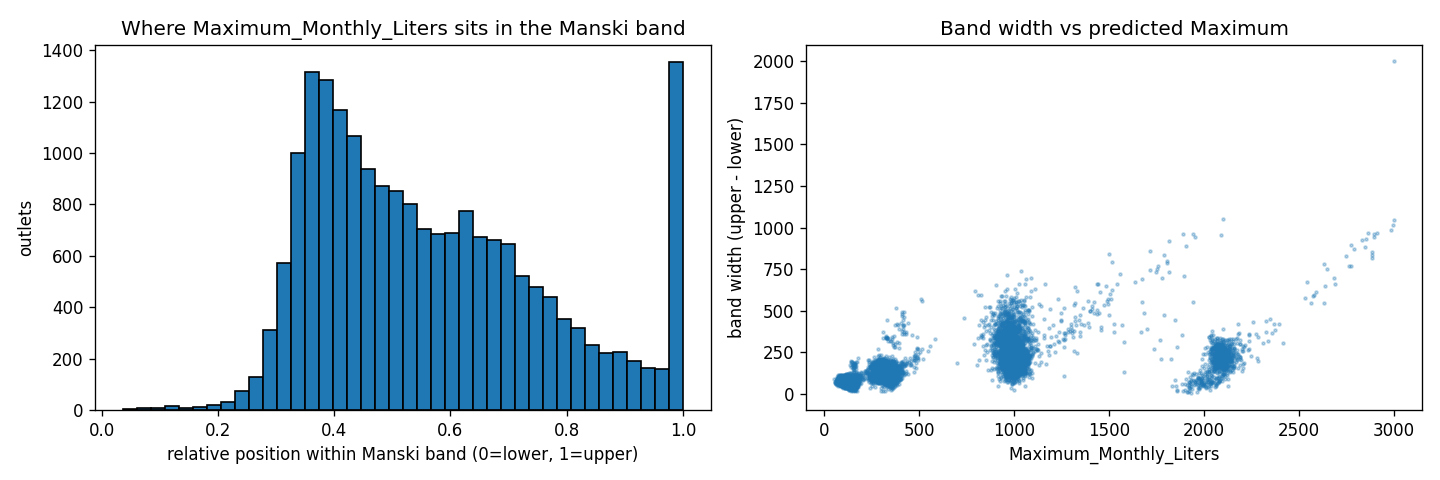
\includegraphics[width=\textwidth]{eda_manski_band.png}
\caption{Per-outlet Manski band around the submitted point.}
\end{subfigure}\hfill
\begin{subfigure}{0.49\textwidth}\centering
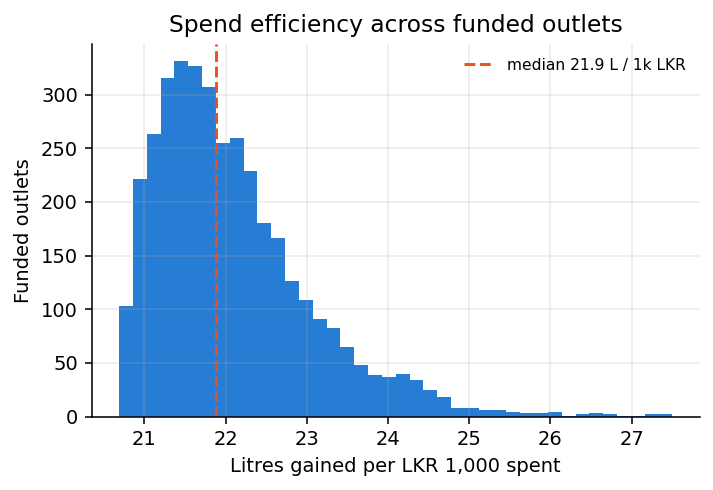
\includegraphics[width=\textwidth]{fr_spend_efficiency.png}
\caption{Litres gained per LKR 1,000 across funded outlets.}
\end{subfigure}
\caption{Uncertainty disclosure (left) and spend efficiency (right).}
\end{figure}

\subsection{Outlet Intelligence web app}
A local \textbf{Streamlit} app (\texttt{app/streamlit\_app.py}, no external
services) with three tabs: \textbf{Browse} (filter by province/distributor/type,
search, map, CSV export), \textbf{Drill-down} (per-outlet metrics, signed
drivers, on-demand XAI narrative with live/offline toggle, raw payload), and
\textbf{Western spend plan} (the LKR 5M allocation with utilisation, funded count,
expected uplift, and submission download).

% =============================================================================
\section{GenAI Transparency Log}
\begin{table}[H]
\centering\footnotesize
\begin{tabularx}{\textwidth}{lYY}
\toprule
\textbf{Phase} & \textbf{AI usage} & \textbf{Human validation}\\
\midrule
Research swarm & 10-channel parallel research swarm $\rightarrow$ research brief & each claim cross-checked vs cited URLs\\
Methodology audit & 7 rounds of 4--5 parallel critics (Statistician, Skeptic, Architect, DE, Gap, Judge, Risk) & every finding cites \texttt{file:line}; verified / rebutted\\
Code + design & JLMS closed form; OSM tag survey; Geofabrik vs Overpass; KKT derivation & syntax / import checks; SFA vs Greene; optimizer proven concave\\
XAI integration & narrative prompt engineering; driver schema design & narratives validated vs structured drivers; offline tested\\
Report drafting & LaTeX assembly + content port from markdown & every claim traced to \texttt{Results/} or \texttt{data/gold/}\\
\bottomrule
\end{tabularx}
\caption{Per-phase GenAI transparency. Full log:
\texttt{Docs/ai\_transparency\_log.md} (R1--R7 audit trail).}
\end{table}

\subsection*{Deliverables}
\begin{table}[H]
\centering\small
\begin{tabularx}{\textwidth}{lY}
\toprule
\textbf{Artifact} & \textbf{Path}\\
\midrule
Platform predictions CSV & \texttt{Results/smile\_labs\_predictions.csv} (20,000 rows)\\
Budget allocations CSV & \texttt{Results/smile\_labs\_budget\_allocations.csv}\\
Manski + conformal bands & \texttt{Results/manski\_bands\_v2.csv}, \texttt{conformal\_intervals\_v2.csv}\\
Validation & \texttt{Results/validation\_report.md} (6/6 PASS)\\
Outlet Intelligence app & \texttt{app/streamlit\_app.py}\\
Reproducible codebase & \texttt{run\_pipeline.py} + \texttt{run\_final\_round.py}; \texttt{src/}\\
\bottomrule
\end{tabularx}
\end{table}

% =============================================================================
\begin{thebibliography}{9}
\small
\bibitem{manski} C. F. Manski. \emph{Partial Identification of Probability Distributions.} Springer, 2003.
\bibitem{sfa} D. Aigner, C. A. K. Lovell, P. Schmidt. Formulation and Estimation of Stochastic Frontier Production Function Models. \emph{J. Econometrics} 6.1 (1977).
\bibitem{jlms} J. Jondrow et al. On the Estimation of Technical Inefficiency in the SFA Model. \emph{J. Econometrics} 19.2--3 (1982).
\bibitem{ch} V. Chernozhukov, H. Hong. Three-Step Censored Quantile Regression. \emph{JASA} 97.459 (2002).
\bibitem{cqr} Y. Romano, E. Patterson, E. J. Cand\`es. Conformalized Quantile Regression. \emph{NeurIPS} 32 (2019).
\bibitem{geofabrik} Geofabrik GmbH. OpenStreetMap Data Extracts -- Sri Lanka. Accessed Jan 2026.
\bibitem{xgb} T. Chen, C. Guestrin. XGBoost: A Scalable Tree Boosting System. \emph{KDD '16} (2016).
\bibitem{cfg} V. Chernozhukov, I. Fern\'andez-Val, A. Galichon. Quantile and Probability Curves Without Crossing. \emph{Econometrica} 78.3 (2010).
\bibitem{powell} J. L. Powell. Censored Regression Quantiles. \emph{J. Econometrics} 32.1 (1986).
\end{thebibliography}

\end{document}
